% Source: src-8d14b1f9f511665ea10dbda45959a3b445a17806415be6b034f816bec663d7f5
% PDF SHA-256: 35e5d6f6bf052fcd9a2b91a1aa4215766fd4121425cfec7a62cfc4cdc7ab02a1
% PDF page 1, printed page 72, question 18. Schematic topology only; no metric properties are inferred.
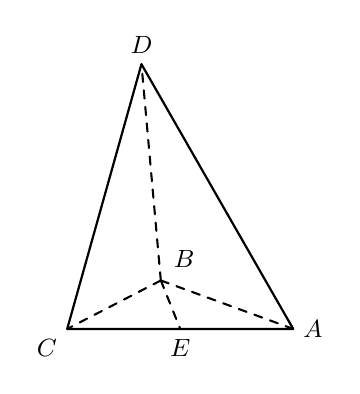
\begin{tikzpicture}[x=0.82cm,y=0.82cm,line cap=round,line join=round,line width=0.75pt,font=\small]
  \coordinate (A) at (3.5,0);
  \coordinate (B) at (1.45,0.75);
  \coordinate (C) at (0,0);
  \coordinate (D) at (1.15,4.1);
  \coordinate (E) at (1.75,0);
  \draw[thick] (C)--(D)--(A)--(C);
  \draw[dashed] (B)--(A) (B)--(C) (B)--(D) (B)--(E);
  \node[above] at (D) {$D$};
  \node[above right=1pt] at (B) {$B$};
  \node[below left] at (C) {$C$};
  \node[right] at (A) {$A$};
  \node[below] at (E) {$E$};
\end{tikzpicture}
